	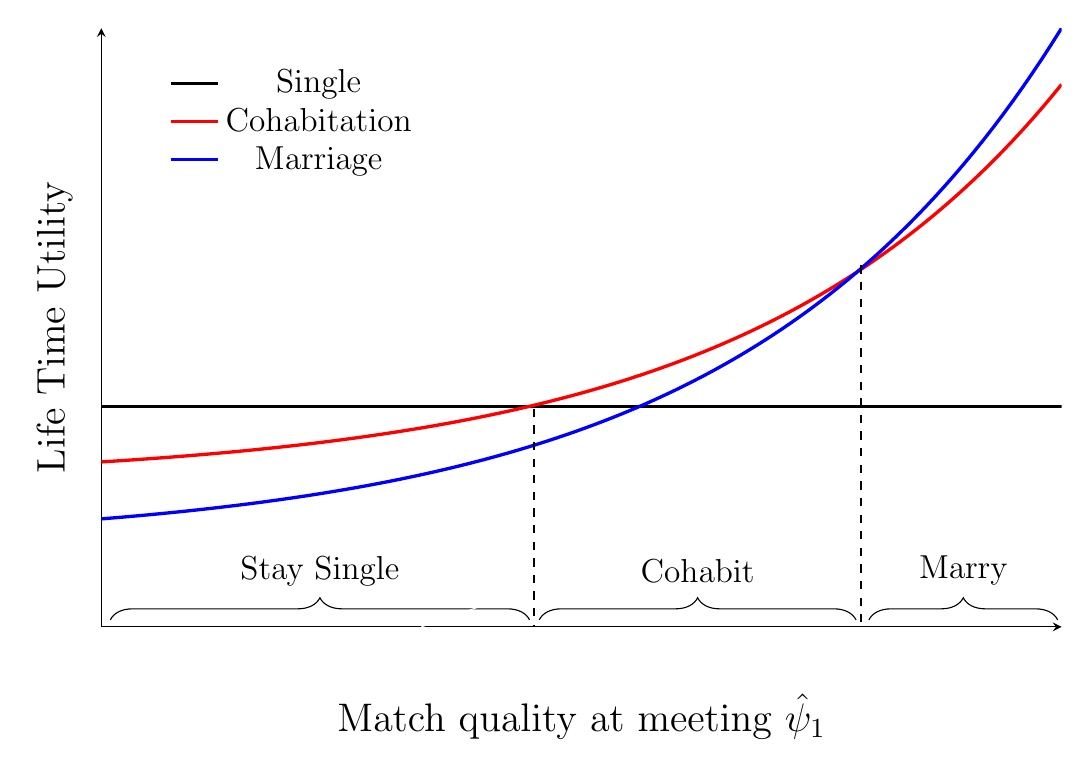
\begin{tikzpicture}[thick,scale=1]
	\begin{axis}[
	width=278.0*1.5*0.94,
    height=278.0*0.94,
	ticks=none,
	yticklabels={,,},
	xticklabels={,,},
	legend columns=1, 
	x label style={at={(axis description cs:0.5,-0.095)},anchor=north},
	y label style={at={(axis description cs:-0.02,.5)},anchor=south},
	legend style={font=\large},
	axis lines = left,
	xlabel = {\Large{Match quality at meeting $\hat{\psi}_1$}},
	ylabel = {\Large{Life Time Utility}},
	legend style={at={(0.2,+0.95)},anchor=north,draw=none}
	]
	
	%%%%%%%%%%%%%%%%%%
	%Here The Envelop
	%%%%%%%%%%%%%%%%%%

	%Brace Single
	\draw [decorate,decoration={brace,amplitude=8pt,mirror,raise=5pt},xshift=-65pt,yshift=15pt]
	 (0.90,0.0)--(-0.41,0.0)  node [black,midway,xshift=0cm,yshift=0.8cm] {\large Stay Single};
	
	%Brace Cohabitation
	\draw [decorate,decoration={brace,amplitude=8pt,mirror,raise=5pt},xshift=-65pt,yshift=15pt]
	(1.92,0.0) -- (0.93,0.00) node [black,midway,xshift=0cm,yshift=0.8cm] {\large Cohabit};
	
	%Brace Marriage
	\draw [decorate,decoration={brace,amplitude=8pt,mirror,raise=5pt},xshift=-65pt,yshift=15pt]
	(2.55,0)--(1.96,0) node [black,midway,xshift=0cm,yshift=0.8cm] {\large Marry};
	
	%Just for the style
	\addplot [
	domain=0:2, 
	color=white,
	style=thin,forget plot
	%	mark=star,
	%	mark repeat=15,
	%	mark phase=5
	]
	{0.90000001+2.04*x+0.2*x^2-0.09*x^3};	
	
	
	
	
	
	%Below the red parabola is defined
	\addplot [
	domain=-1:2, 
	samples=100, 
	color=black,
	style=very thick,
	]
	{5+0.0000000002*x};
	\addlegendentry{Single}
	
	\addplot [
	domain=-1.0:2, 
	samples=100, 
	color=red,
	style=very thick,
	%		mark=triangle*,
	%		mark repeat=15,
	%		mark phase=5
	]
	{exp(x)+3.6};
	\addlegendentry{Cohabitation}
	
	\addplot [
	domain=-1.0:2, 
	samples=100, 
	color=blue,
	style=solid,
	style=very thick,
	mark phase=5
	]
	{1.3*exp(x)+2.43};
	\addlegendentry{Marriage}
	
	
	\end{axis}
	
	%Here I add the label of the points
\draw [dashed] (5.5,2.77)
-- (5.5,0);

\draw [dashed,] (9.65,4.59)
-- (9.65,0);
	\end{tikzpicture}